\documentclass[aspectratio=169, 10pt]{beamer}

% --- Packages ---
\usepackage[utf8]{inputenc}
\usepackage{tikz}
\usepackage{pgfplots}
\usepackage{amsmath, amssymb, amsfonts}
\usepackage{booktabs}
\usepackage{bm}
\usepackage{xcolor}
\usetikzlibrary{arrows.meta, calc, positioning, shapes.geometric, decorations.pathreplacing, backgrounds, fit, shadows, patterns, shapes.arrows, angles, quotes}
\pgfplotsset{compat=1.17}

% NYU Colors
\definecolor{nyupurple}{RGB}{87,46,140}
\definecolor{nyuheader}{RGB}{172,159,195}
\definecolor{nyufooter}{RGB}{189,178,211}

% Theme
\usetheme{default}
\setbeamertemplate{navigation symbols}{}

% Itemize
\setbeamercolor{itemize item}{fg=nyupurple}
\setbeamercolor{itemize subitem}{fg=nyupurple}
\setbeamercolor{itemize subsubitem}{fg=nyupurple}
\setbeamertemplate{itemize item}{\textbullet}
\setbeamertemplate{itemize subitem}{\textbullet}
\setbeamertemplate{itemize subsubitem}{\textbullet}

% Blocks
\setbeamercolor{block title}{fg=white, bg=nyupurple}
\setbeamercolor{block body}{fg=black, bg=nyuheader!30}
\setbeamercolor{block title alerted}{fg=white, bg=red!70}
\setbeamercolor{block body alerted}{fg=black, bg=red!10}
\setbeamercolor{block title example}{fg=white, bg=green!50!black}
\setbeamercolor{block body example}{fg=black, bg=green!10}

% Diagram colors
\definecolor{darkblue}{RGB}{0,51,102}
\definecolor{brightblue}{RGB}{0,102,204}
\definecolor{lightblue}{RGB}{153,204,255}
\definecolor{darkgreen}{RGB}{0,102,51}
\definecolor{accentred}{RGB}{192,0,0}
\definecolor{accentgreen}{RGB}{0,128,0}
\definecolor{accentorange}{RGB}{255,128,0}

% Commands
\newcommand{\vect}[1]{\boldsymbol{#1}}
\newcommand{\mat}[1]{\mathbf{#1}}

% Header
\makeatletter
\setbeamertemplate{frametitle}{%
    \nointerlineskip%
    \begin{beamercolorbox}[wd=\paperwidth,ht=0.7cm,dp=0.15cm,rightskip=0.5cm]{frametitle}
        \hspace{0.3cm}\usebeamerfont{frametitle}\insertframetitle%
        \hfill%
        \raisebox{0.08cm}{{\bfseries\sffamily\color{nyupurple}NYU}}%
    \end{beamercolorbox}%
}
\makeatother
\setbeamercolor{frametitle}{fg=black, bg=nyuheader}
\setbeamerfont{frametitle}{size=\large}

% Footer
\setbeamertemplate{footline}{%
    \begin{tikzpicture}[remember picture, overlay]
        \fill[nyufooter] ([yshift=0.6cm]current page.south west) rectangle ([xshift=5cm]current page.south east);
        \fill[nyufooter!70] ([yshift=0.6cm, xshift=5cm]current page.south west) rectangle ([xshift=10.5cm]current page.south east);
        \fill[nyufooter!40] ([yshift=0.6cm, xshift=10.5cm]current page.south west) rectangle (current page.south east);
        \node[anchor=west, font=\small] at ([xshift=0.3cm, yshift=0.3cm]current page.south west) {Dr.\ Aliasghar Arab};
        \node[anchor=center, font=\small] at ([yshift=0.3cm]current page.south) {Autonomous Mobile Robots};
        \node[anchor=east, font=\small] at ([xshift=-0.3cm, yshift=0.3cm]current page.south east) {LECTURE 9 -- FALL 2025 \quad \insertframenumber{} / \inserttotalframenumber};
    \end{tikzpicture}%
}

% Title page
\defbeamertemplate*{title page}{customized}[1][]
{
    \begin{tikzpicture}[remember picture, overlay]
        \node[anchor=north east] at ([xshift=-0.8cm, yshift=-0.8cm]current page.north east) {%
            {\bfseries\sffamily\Large\color{nyupurple}NYU}%
            {\sffamily\normalsize\color{black}\ \ TANDON SCHOOL OF ENGINEERING}%
        };
    \end{tikzpicture}
    
    \vspace{2cm}
    \centering
    {\Large\bfseries\inserttitle\par}
    \vspace{0.3cm}
    {\insertsubtitle\par}
    \vspace{1cm}
    {\insertauthor\par}
    \vspace{0.3cm}
    {\small\insertinstitute\par}
    \vspace{0.5cm}
    {\insertdate\par}
}

% Title info
\title{Autonomous Mobile Robots}
\subtitle{Lecture 9: Planning Methods Review}
\author{Dr.\ Aliasghar Arab}
\institute{NYU Tandon School of Engineering}
\date{Fall 2025}

\begin{document}

% ============================================================================
% TITLE SLIDE
% ============================================================================
{
\setbeamertemplate{footline}{}
\begin{frame}[plain]
\titlepage
\end{frame}
}

% ============================================================================
% INTRODUCTION
% ============================================================================

\begin{frame}{Today's Objective}
\begin{itemize}
\item Review main planning methods we've covered
\item Understand how planning evolved from industrial robotics
\item See how different approaches solve the same problem
\item Connect planning to the full robotic system architecture
\end{itemize}
\end{frame}

\begin{frame}{The Fundamental Division}
\begin{alertblock}{Core Distinction}
How they construct the configuration space for search
\end{alertblock}

\vspace{0.4cm}

\begin{columns}[T]
\column{0.48\textwidth}
\begin{block}{Probabilistic Planning}
\begin{itemize}
\item Random sampling of configuration space
\item Example: RRT (Rapidly-exploring Random Trees)
\item No explicit graph construction
\item Explores through randomness
\end{itemize}
\end{block}

\column{0.48\textwidth}
\begin{block}{Deterministic Planning}
\begin{itemize}
\item Systematic graph construction
\item Then search the graph
\item Explicit discretization
\item Methodical exploration
\end{itemize}
\end{block}
\end{columns}
\end{frame}

\begin{frame}{The Planning Problem}
\begin{block}{Mathematical Formulation}
\textbf{Given:}
\begin{itemize}
\item Starting configuration: $q_0 = q_i$ (initial)
\item Goal configuration: $q_n = q_{des}$ (desired)
\end{itemize}

\vspace{0.3cm}

\textbf{Find:} A sequence of points
\[Q = \{q_0, q_1, q_2, \ldots, q_n\}\]

That connects the robot from start to goal without collisions
\end{block}

\vspace{0.3cm}

\begin{center}
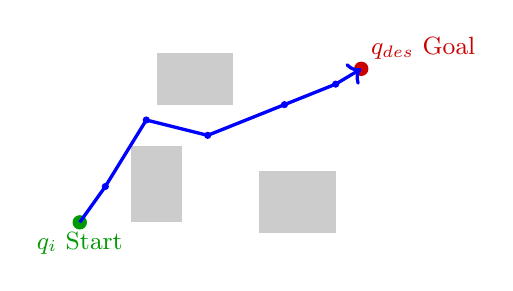
\begin{tikzpicture}[scale=0.65]
% Obstacles
\fill[gray!40] (1.5,0.5) rectangle (2.5,2);
\fill[gray!40] (4,0.3) rectangle (5.5,1.5);
\fill[gray!40] (2,2.8) rectangle (3.5,3.8);

% Start and Goal
\fill[green!60!black] (0.5,0.5) circle (4pt) node[below, font=\small] {$q_i$ Start};
\fill[red!80!black] (6,3.5) circle (4pt) node[above right, font=\small] {$q_{des}$ Goal};

% Path
\draw[blue, very thick, ->] (0.5,0.5) -- (1,1.2) -- (1.8,2.5) -- (3,2.2) -- (4.5,2.8) -- (5.5,3.2) -- (6,3.5);

% Points on path
\foreach \point in {(1,1.2), (1.8,2.5), (3,2.2), (4.5,2.8), (5.5,3.2)} {
    \fill[blue] \point circle (2pt);
}
\end{tikzpicture}
\end{center}
\end{frame}

% ============================================================================
% PROBABILISTIC PLANNING
% ============================================================================

\begin{frame}{Probabilistic Planning: RRT Review}
\begin{block}{Rapidly-exploring Random Trees (RRT)}
\textbf{Mechanism:}
\begin{enumerate}
\item Start from initial point
\item Generate random nodes
\item Connect to nearest node
\item Grow toward unexplored regions
\end{enumerate}
\end{block}

\vspace{0.2cm}

\begin{center}
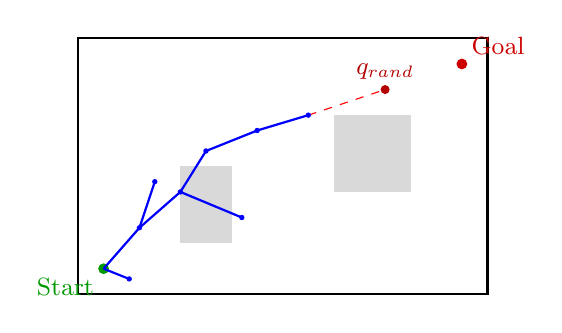
\begin{tikzpicture}[scale=0.65]
% Boundary
\draw[thick] (0,0) rectangle (8,5);

% Obstacles
\fill[gray!30] (2,1) rectangle (3,2.5);
\fill[gray!30] (5,2) rectangle (6.5,3.5);

% Start
\fill[green!60!black] (0.5,0.5) circle (3pt) node[below left, font=\small] {Start};

% Tree structure
\draw[blue, thick] (0.5,0.5) -- (1.2,1.3);
\draw[blue, thick] (0.5,0.5) -- (1,0.3);
\draw[blue, thick] (1.2,1.3) -- (2,2);
\draw[blue, thick] (2,2) -- (2.5,2.8);
\draw[blue, thick] (2.5,2.8) -- (3.5,3.2);
\draw[blue, thick] (3.5,3.2) -- (4.5,3.5);
\draw[blue, thick] (2,2) -- (3.2,1.5);
\draw[blue, thick] (1.2,1.3) -- (1.5,2.2);

% Random sample
\fill[red!70!black] (6,4) circle (2.5pt) node[above, font=\small] {$q_{rand}$};
\draw[red, dashed] (4.5,3.5) -- (6,4);

% Nodes
\foreach \point in {(1.2,1.3), (1,0.3), (2,2), (2.5,2.8), (3.5,3.2), (4.5,3.5), (3.2,1.5), (1.5,2.2)} {
    \fill[blue] \point circle (1.5pt);
}

% Goal
\fill[red!80!black] (7.5,4.5) circle (3pt) node[above right, font=\small] {Goal};
\end{tikzpicture}
\end{center}

\vspace{0.2cm}

\begin{alertblock}{Key Feature}
Probabilistic sampling - no explicit map needed
\end{alertblock}
\end{frame}

\begin{frame}{Probabilistic Completeness}
\begin{block}{Theoretical Guarantee}
\textbf{PROBABILISTIC COMPLETENESS:}

If time goes to infinity, the algorithm will converge to a solution
\end{block}

\vspace{0.3cm}

\begin{columns}[T]
\column{0.48\textwidth}
\begin{exampleblock}{The Promise}
\begin{itemize}
\item Path will eventually be found
\item Probability $\to$ 1.0 as samples $\to \infty$
\item No explicit discretization
\end{itemize}
\end{exampleblock}

\column{0.48\textwidth}
\begin{alertblock}{The Issue}
\textit{"There is no time limited"}
\begin{itemize}
\item Convergence in infinite time
\item No finite time guarantee
\item Unpredictable solution time
\end{itemize}
\end{alertblock}
\end{columns}

\vspace{0.3cm}

\begin{block}{Comparison}
\textit{"Deterministic methods can at least guarantee convergence in a limited time"}
\end{block}
\end{frame}

\begin{frame}{When to Use Probabilistic Methods?}
\begin{columns}[T]
\column{0.48\textwidth}
\begin{block}{Advantages}
\begin{itemize}
\item High-dimensional spaces
\item 6+ DOF robot arms
\item No explicit free-space map
\item Proven completeness
\end{itemize}
\end{block}

\column{0.48\textwidth}
\begin{block}{Disadvantages}
\begin{itemize}
\item Convergence time $\to \infty$
\item No finite time guarantee
\item Non-repeatable paths
\item Random variance
\end{itemize}
\end{block}
\end{columns}

\vspace{0.3cm}

\begin{exampleblock}{Application Context}
\textit{"Based on the situations and the problem you are solving, there might be good enough methods to use for your specific problem. You don't need to go look into more complex methods such as RRT."}
\end{exampleblock}
\end{frame}

% ============================================================================
% DETERMINISTIC PLANNING
% ============================================================================

\begin{frame}{Deterministic Planning Framework}
\begin{block}{General Deterministic Planning - Two Steps}
\textbf{STEP 1: CONSTRUCT A GRAPH}
\begin{itemize}
\item Create nodes (V) - discrete configuration samples
\item Create edges (E) - valid connections between nodes
\item Discretize the continuous configuration space
\end{itemize}

\vspace{0.3cm}

\textbf{STEP 2: GRAPH SEARCH}
\begin{itemize}
\item Find optimal path from start to goal
\item Use standard graph search algorithms
\item Guarantee bounded time solution
\end{itemize}
\end{block}

\vspace{0.3cm}

\begin{alertblock}{Key Advantage}
\textit{"Can guarantee we will converge in a limited time"}
\end{alertblock}
\end{frame}

\begin{frame}{Why Deterministic for Mobile Robots?}
\begin{exampleblock}{Dimensional Advantage}
Mobile robots: 2D/3D navigation (3-6 DOF)\\
Manipulators: 6-20+ DOF
\end{exampleblock}

\vspace{0.3cm}

\begin{block}{Engineering Trade-off}
\begin{itemize}
\item Lower dimensions $\to$ deterministic feasible
\item More straightforward than RRT
\item Repeatable, optimal solutions
\end{itemize}
\end{block}
\end{frame}

\begin{frame}{Graph Construction Challenge}
\begin{block}{The Question}
\textit{"What places do you recommend to put nodes?"}
\end{block}

\vspace{0.3cm}

\begin{center}
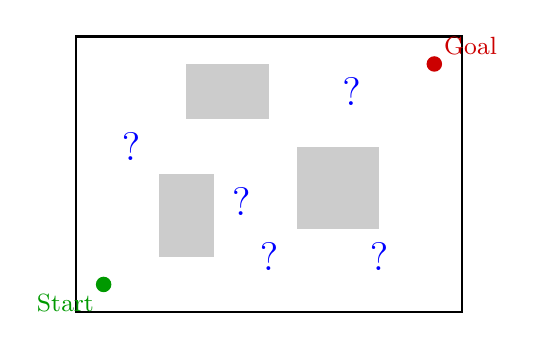
\begin{tikzpicture}[scale=0.7]
% Boundary
\draw[thick] (0,0) rectangle (7,5);

% Obstacles
\fill[gray!40] (1.5,1) rectangle (2.5,2.5);
\fill[gray!40] (4,1.5) rectangle (5.5,3);
\fill[gray!40] (2,3.5) rectangle (3.5,4.5);

% Start and Goal
\fill[green!60!black] (0.5,0.5) circle (4pt) node[below left, font=\small] {Start};
\fill[red!80!black] (6.5,4.5) circle (4pt) node[above right, font=\small] {Goal};

% Question marks
\node[blue, font=\Large] at (1,3) {?};
\node[blue, font=\Large] at (3,2) {?};
\node[blue, font=\Large] at (5,4) {?};
\node[blue, font=\Large] at (5.5,1) {?};
\node[blue, font=\Large] at (3.5,1) {?};
\end{tikzpicture}
\end{center}

\vspace{0.2cm}

\begin{center}
\textbf{Where should we place nodes?}
\end{center}
\end{frame}

% ============================================================================
% GRAPH CONSTRUCTION METHODS
% ============================================================================

\begin{frame}{Method 1: Visibility Graphs}
\begin{block}{Construction Approach}
\textbf{Place nodes at obstacle vertices (corners)}

\begin{itemize}
\item Connect nodes if line of sight is clear
\item No edge through obstacles
\item Include start and goal
\end{itemize}
\end{block}

\vspace{0.2cm}

\begin{center}
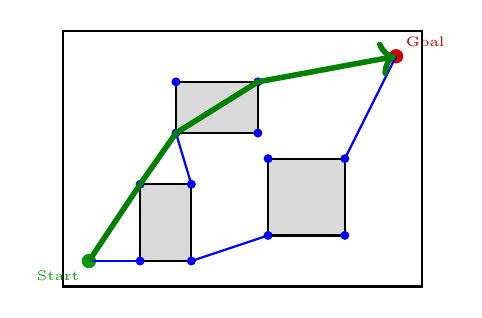
\begin{tikzpicture}[scale=0.65]
% Obstacles with vertices
\draw[fill=gray!30, thick] (1.5,0.5) -- (2.5,0.5) -- (2.5,2) -- (1.5,2) -- cycle;
\draw[fill=gray!30, thick] (4,1) -- (5.5,1) -- (5.5,2.5) -- (4,2.5) -- cycle;
\draw[fill=gray!30, thick] (2.2,3) -- (3.8,3) -- (3.8,4) -- (2.2,4) -- cycle;

% Vertices as nodes
\foreach \point in {(1.5,0.5), (2.5,0.5), (2.5,2), (1.5,2), (4,1), (5.5,1), (5.5,2.5), (4,2.5), (2.2,3), (3.8,3), (3.8,4), (2.2,4)} {
    \fill[blue] \point circle (2.5pt);
}

% Start and Goal
\fill[green!60!black] (0.5,0.5) circle (4pt) node[below left, font=\tiny] {Start};
\fill[red!80!black] (6.5,4.5) circle (4pt) node[above right, font=\tiny] {Goal};

% Sample edges
\draw[blue, thick] (0.5,0.5) -- (1.5,0.5);
\draw[blue, thick] (0.5,0.5) -- (1.5,2);
\draw[blue, thick] (2.5,0.5) -- (4,1);
\draw[blue, thick] (2.5,2) -- (2.2,3);
\draw[blue, thick] (3.8,4) -- (6.5,4.5);
\draw[blue, thick] (5.5,2.5) -- (6.5,4.5);

% Optimal path
\draw[green!50!black, line width=2pt, ->] (0.5,0.5) -- (1.5,2) -- (2.2,3) -- (3.8,4) -- (6.5,4.5);

% Boundary
\draw[thick] (0,0) rectangle (7,5);
\end{tikzpicture}
\end{center}

\vspace{0.2cm}

\begin{alertblock}{Result}
Paths along obstacle boundaries - optimal length
\end{alertblock}
\end{frame}

\begin{frame}{Visibility Graphs: The ``Touching the Wall'' Problem}
\begin{alertblock}{Critical Flaw}
\textit{"Only the nodes that can be connected with no collision"}

BUT: The optimal path grazes very close to obstacle edges
\end{alertblock}

\vspace{0.3cm}

\begin{columns}[T]
\column{0.55\textwidth}
\begin{block}{Why This Matters}
\begin{itemize}
\item Real robots have uncertainty
\item Sensor noise
\item Controller imperfection
\item Localization errors
\end{itemize}

\textit{``Touching wall'' = collision risk}
\end{block}

\column{0.4\textwidth}
\begin{center}
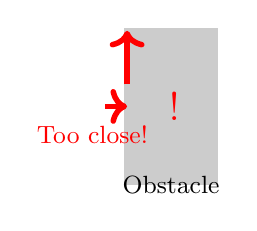
\begin{tikzpicture}[scale=0.8]
\fill[gray!40] (0,0) rectangle (1.5,2.5);

\draw[red, line width=2pt, ->] (-0.3,1.25) -- (0.05,1.25);
\draw[red, line width=2pt, ->] (0.05,1.6) -- (0.05,2.45);

\node[red, font=\small] at (-0.5,0.8) {Too close!};
\node[red, font=\Large] at (0.8,1.25) {!};

\node[font=\small] at (0.75,0) {Obstacle};
\end{tikzpicture}
\end{center}
\end{columns}

\vspace{0.3cm}

\begin{exampleblock}{Solution}
Inflate obstacles by robot radius (add buffer)
\end{exampleblock}
\end{frame}

\begin{frame}{Visibility Graphs: Round Obstacle Challenge}
\begin{block}{Engineering Problem}
\textit{"You have to come up with some engineering solution..."}
\end{block}

\vspace{0.3cm}

\begin{center}
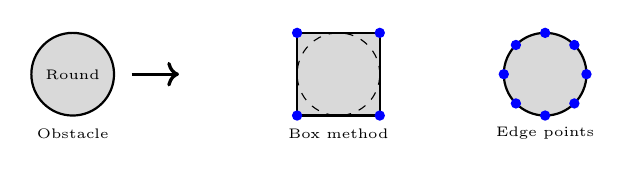
\begin{tikzpicture}[scale=0.75]
% Original round obstacle
\draw[fill=gray!30, thick] (2,2) circle (0.7);
\node[font=\tiny] at (2,2) {Round};
\node[font=\tiny] at (2,1) {Obstacle};

% Arrow
\draw[->, very thick] (3,2) -- (3.8,2);

% Option 1: Box
\begin{scope}[xshift=4.5cm]
\draw[fill=gray!30, thick] (1.3,1.3) rectangle (2.7,2.7);
\draw[dashed] (2,2) circle (0.7);
\node[font=\tiny] at (2,1) {Box method};
\foreach \point in {(1.3,1.3), (2.7,1.3), (2.7,2.7), (1.3,2.7)} {
    \fill[blue] \point circle (2.5pt);
}
\end{scope}

% Option 2: Edge points
\begin{scope}[xshift=8cm]
\draw[fill=gray!30, thick] (2,2) circle (0.7);
\node[font=\tiny] at (2,1) {Edge points};
\foreach \angle in {0,45,90,135,180,225,270,315} {
    \fill[blue] (2+0.7*cos \angle,2+0.7*sin \angle) circle (2.5pt);
}
\end{scope}
\end{tikzpicture}
\end{center}

\vspace{0.3cm}

\begin{alertblock}{Challenge}
\textit{"Finding exact points on circle edges is computationally challenging"}
\end{alertblock}
\end{frame}

\begin{frame}{Method 2: Voronoi Diagrams}
\begin{block}{Voronoi Approach}
\textbf{Nodes in the middle of free space between obstacles}

\vspace{0.2cm}

\textbf{Key Property:}
\begin{itemize}
\item Points equidistant from multiple obstacles
\item Creates ``roads'' through free space
\item Maximizes clearance from walls
\end{itemize}
\end{block}

\vspace{0.2cm}

\begin{center}
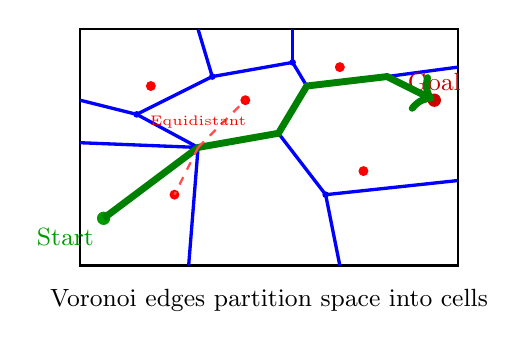
\begin{tikzpicture}[scale=0.6]
% Boundary
\draw[thick] (0,0) rectangle (8,5);

% Obstacles (sites) - red dots
\fill[red] (2,1.5) circle (3pt);
\fill[red] (3.5,3.5) circle (3pt);
\fill[red] (6,2) circle (3pt);
\fill[red] (1.5,3.8) circle (3pt);
\fill[red] (5.5,4.2) circle (3pt);

% Voronoi edges (blue lines forming cell boundaries)
\draw[blue, very thick] (0,2.6) -- (2.5,2.5) -- (4.2,2.8);
\draw[blue, very thick] (2.5,2.5) -- (2.3,0);
\draw[blue, very thick] (2.5,2.5) -- (1.2,3.2);
\draw[blue, very thick] (1.2,3.2) -- (0,3.5);
\draw[blue, very thick] (1.2,3.2) -- (2.8,4);
\draw[blue, very thick] (2.8,4) -- (4.5,4.3);
\draw[blue, very thick] (4.5,4.3) -- (4.5,5);
\draw[blue, very thick] (2.8,4) -- (2.5,5);
\draw[blue, very thick] (4.2,2.8) -- (4.8,3.8);
\draw[blue, very thick] (4.8,3.8) -- (4.5,4.3);
\draw[blue, very thick] (4.2,2.8) -- (5.2,1.5);
\draw[blue, very thick] (5.2,1.5) -- (5.5,0);
\draw[blue, very thick] (5.2,1.5) -- (8,1.8);
\draw[blue, very thick] (4.8,3.8) -- (6.5,4);
\draw[blue, very thick] (6.5,4) -- (8,4.2);

% Voronoi vertices (where edges meet)
\foreach \point in {(2.5,2.5), (1.2,3.2), (2.8,4), (4.5,4.3), (4.2,2.8), (5.2,1.5), (4.8,3.8), (6.5,4)} {
    \fill[blue] \point circle (2pt);
}

% Start and Goal
\fill[green!60!black] (0.5,1) circle (4pt) node[below left, font=\small] {Start};
\fill[red!80!black] (7.5,3.5) circle (4pt) node[above, font=\small] {Goal};

% Example path following Voronoi edges
\draw[green!50!black, line width=2.5pt, ->] (0.5,1) -- (2.5,2.5) -- (4.2,2.8) -- (4.8,3.8) -- (6.5,4) -- (7.5,3.5);

% Show equal distance at one point
\draw[red!70, dashed, thick] (2.5,2.5) -- (2,1.5);
\draw[red!70, dashed, thick] (2.5,2.5) -- (3.5,3.5);
\node[red, above, font=\tiny] at (2.5,2.7) {Equidistant};

\node[below, font=\small, align=center] at (4,-0.3) {Voronoi edges partition space into cells};
\end{tikzpicture}
\end{center}
\end{frame}

\begin{frame}{Voronoi Diagrams: Safety vs Optimality}
\begin{columns}[T]
\column{0.52\textwidth}
\begin{block}{ADVANTAGE: Safety}
\textit{"Good advantage is uncertainty in obstacle locations and not going sharply from edges"}

\vspace{0.2cm}

\begin{itemize}
\item Maximizes clearance
\item Handles localization uncertainty
\item Safer paths
\end{itemize}
\end{block}

\column{0.45\textwidth}
\begin{alertblock}{DISADVANTAGE: Path Length}
\textit{"The main issue is the optimality"}

\vspace{0.2cm}

\begin{itemize}
\item Longer paths
\item Takes ``scenic route''
\item Not near optimal
\end{itemize}
\end{alertblock}
\end{columns}

\vspace{0.3cm}

\begin{center}
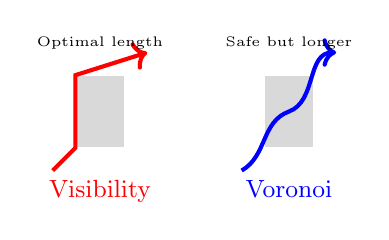
\begin{tikzpicture}[scale=0.6]
% Visibility path
\begin{scope}
\fill[gray!30] (0.5,0.5) rectangle (1.5,2);
\draw[red, line width=1.5pt, ->] (0,0) -- (0.48,0.48) -- (0.48,2.02) -- (2,2.5);
\node[red, below] at (1,0) {\small Visibility};
\node[font=\tiny] at (1,2.7) {Optimal length};
\end{scope}

% Voronoi path
\begin{scope}[xshift=4cm]
\fill[gray!30] (0.5,0.5) rectangle (1.5,2);
\draw[blue, line width=1.5pt, ->] (0,0) to[out=30,in=200] (1,1.25) to[out=20,in=180] (2,2.5);
\node[blue, below] at (1,0) {\small Voronoi};
\node[font=\tiny] at (1,2.7) {Safe but longer};
\end{scope}
\end{tikzpicture}
\end{center}
\end{frame}

\begin{frame}{Method 3: Cell Decomposition}
\begin{block}{Grid-Based Approach}
\textit{"Excel Cell Decomposition" - Exact Cell Decomposition}

\begin{itemize}
\item Divide free space into cells
\item Cell centers $\to$ nodes
\item Adjacent cells $\to$ edges
\end{itemize}
\end{block}

\vspace{0.2cm}

\begin{center}
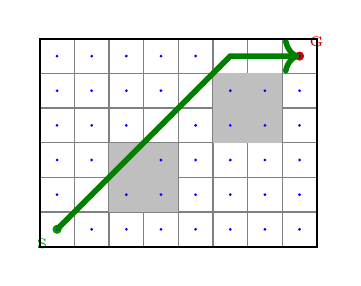
\begin{tikzpicture}[scale=0.55]
% Grid
\draw[step=0.8,gray,thin] (0,0) grid (6.4,4.8);

% Obstacles
\foreach \x/\y in {1.6/0.8, 2.4/0.8, 1.6/1.6, 2.4/1.6, 4/2.4, 4.8/2.4, 4/3.2, 4.8/3.2} {
    \fill[gray!50] (\x,\y) rectangle ++(0.8,0.8);
}

% Start and Goal
\fill[green!60!black] (0.4,0.4) circle (3pt) node[below left, font=\tiny] {S};
\fill[red!80!black] (6,4.4) circle (3pt) node[above right, font=\tiny] {G};

% Cell centers
\foreach \x in {0.4,1.2,2,2.8,3.6,4.4,5.2,6} {
    \foreach \y in {0.4,1.2,2,2.8,3.6,4.4} {
        \fill[blue] (\x,\y) circle (1pt);
    }
}

% Path
\draw[green!50!black, line width=2pt, ->] (0.4,0.4) -- (1.2,1.2) -- (2,2) -- (2.8,2.8) -- (3.6,3.6) -- (4.4,4.4) -- (5.2,4.4) -- (6,4.4);

\draw[thick] (0,0) rectangle (6.4,4.8);
\end{tikzpicture}
\end{center}

\vspace{0.2cm}

\begin{alertblock}{Limitation}
\textit{"Need to have a full map or construction"}
\end{alertblock}
\end{frame}

\begin{frame}{The Map Dependency Problem}
\begin{alertblock}{Industry Challenge}
\textit{"Having a map is a limitation... I don't think any of them are fully mapless"}
\end{alertblock}

\vspace{0.3cm}

\begin{columns}[T]
\column{0.48\textwidth}
\begin{block}{Current Approach}
Autonomous vehicles:
\begin{itemize}
\item High-definition maps required
\item Construct maps in advance
\item Update maps periodically
\item Expensive operation
\end{itemize}
\end{block}

\column{0.48\textwidth}
\begin{exampleblock}{Industry Examples}
\begin{itemize}
\item \textbf{Wayve} (UK): Claims mapless
\item \textbf{Waymo}: Still uses HD maps
\item \textbf{Most startups}: Hybrid approach
\end{itemize}
\end{exampleblock}
\end{columns}

\vspace{0.3cm}

\begin{block}{The Challenge}
\begin{itemize}
\item Cost of HD map creation and maintenance
\item Computation is still heavy
\end{itemize}
\end{block}
\end{frame}

% ============================================================================
% GRAPH SEARCH ALGORITHMS
% ============================================================================

\begin{frame}{Graph Search Overview}
\begin{block}{Once We Have a Graph...}
Search for optimal path from Start to Goal
\end{block}

\vspace{0.3cm}

\begin{columns}[T]
\column{0.48\textwidth}
\begin{block}{UNINFORMED SEARCH}
No knowledge of goal location

\begin{itemize}
\item Breadth-First Search (BFS)
\item Depth-First Search (DFS)
\end{itemize}

Explore blindly until goal found
\end{block}

\column{0.48\textwidth}
\begin{block}{INFORMED SEARCH}
Use heuristics to guide search

\begin{itemize}
\item Dijkstra's Algorithm
\item A* Search
\item Weighted A*
\end{itemize}

Guide exploration toward goal
\end{block}
\end{columns}
\end{frame}

\begin{frame}{Breadth-First Search (BFS)}
\begin{block}{Level-by-Level Exploration}
\textbf{Mechanism:} Explore all nodes at depth $d$ before $d+1$

\textit{"No Revisit"} - mark nodes to prevent cycles

\vspace{0.2cm}

\textbf{Properties:}
\begin{itemize}
\item $\checkmark$ Complete
\item $\checkmark$ Optimal (unweighted)
\item $\times$ Memory intensive
\end{itemize}
\end{block}

\vspace{0.2cm}

\begin{center}
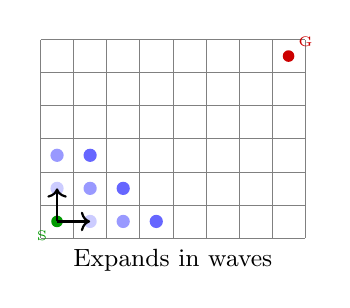
\begin{tikzpicture}[scale=0.7]
\draw[step=0.6,gray,very thin] (0,0) grid (4.8,3.6);

\fill[green!60!black] (0.3,0.3) circle (3pt) node[below left, font=\tiny] {S};

% BFS wavefront
\fill[blue!20] (0.9,0.3) circle (0.12);
\fill[blue!20] (0.3,0.9) circle (0.12);
\fill[blue!40] (1.5,0.3) circle (0.12);
\fill[blue!40] (0.9,0.9) circle (0.12);
\fill[blue!40] (0.3,1.5) circle (0.12);
\fill[blue!60] (2.1,0.3) circle (0.12);
\fill[blue!60] (1.5,0.9) circle (0.12);
\fill[blue!60] (0.9,1.5) circle (0.12);

\fill[red!80!black] (4.5,3.3) circle (3pt) node[above right, font=\tiny] {G};

\draw[->, thick] (0.3,0.3) -- (0.9,0.3);
\draw[->, thick] (0.3,0.3) -- (0.3,0.9);

\node[align=center, font=\small] at (2.4,-0.4) {Expands in waves};
\end{tikzpicture}
\end{center}
\end{frame}

\begin{frame}{Depth-First Search (DFS)}
\begin{block}{Deep Exploration}
\textbf{Mechanism:} \textit{"Explore one path exhaustively"}

\vspace{0.2cm}

\textbf{Properties:}
\begin{itemize}
\item $\checkmark$ Memory efficient
\item $\times$ Not complete (loops)
\item $\times$ Not optimal
\end{itemize}
\end{block}

\vspace{0.2cm}

\begin{center}
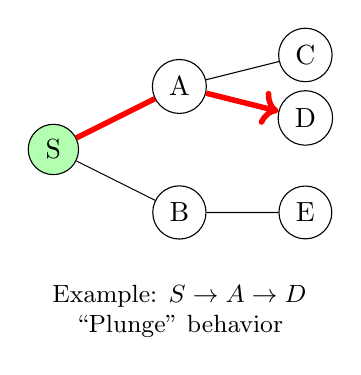
\begin{tikzpicture}[scale=0.8]
% Graph
\node[circle, draw, fill=green!30] (S) at (0,0) {S};
\node[circle, draw] (A) at (2,1) {A};
\node[circle, draw] (B) at (2,-1) {B};
\node[circle, draw] (C) at (4,1.5) {C};
\node[circle, draw] (D) at (4,0.5) {D};
\node[circle, draw] (E) at (4,-1) {E};

\draw (S) -- (A);
\draw (S) -- (B);
\draw (A) -- (C);
\draw (A) -- (D);
\draw (B) -- (E);

% DFS path
\draw[red, line width=2pt, ->] (S) -- (A) -- (D);

\node[below, align=center, font=\small] at (2,-2) {Example: $S \to A \to D$\\``Plunge'' behavior};
\end{tikzpicture}
\end{center}
\end{frame}

\begin{frame}{Cost Functions for Informed Search}
\begin{block}{Key Definitions}
\begin{itemize}
\item $g(n)$ = Cost from Start to node $n$ (actual cost)
\item $h(n)$ = Estimated cost from $n$ to Goal (heuristic)
\item $f(n)$ = Total cost function
\end{itemize}
\end{block}

\vspace{0.2cm}

\begin{center}
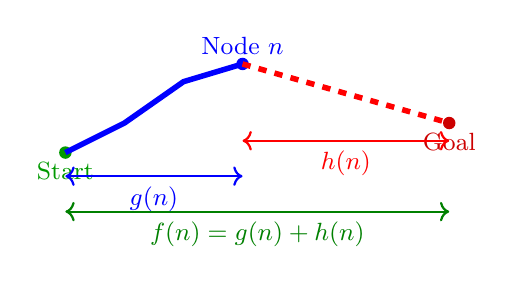
\begin{tikzpicture}[scale=0.75]
\fill[green!60!black] (0,0) circle (3pt) node[below, font=\small] {Start};
\fill[blue] (3,1.5) circle (3pt) node[above, font=\small] {Node $n$};
\fill[red!80!black] (6.5,0.5) circle (3pt) node[below, font=\small] {Goal};

% g(n)
\draw[blue, line width=2pt] (0,0) -- (1,0.5) -- (2,1.2) -- (3,1.5);
\draw[<->, blue, thick] (0,-0.4) -- (3,-0.4) node[midway, below, font=\small] {$g(n)$};

% h(n)
\draw[red, line width=2pt, dashed] (3,1.5) -- (6.5,0.5);
\draw[<->, red, thick] (3,0.2) -- (6.5,0.2) node[midway, below, font=\small] {$h(n)$};

% Total
\draw[<->, green!50!black, thick] (0,-1) -- (6.5,-1) node[midway, below, font=\small] {$f(n) = g(n) + h(n)$};
\end{tikzpicture}
\end{center}

\vspace{0.2cm}

\begin{alertblock}{Implementation}
Heap (Priority Queue) - \textit{"Sorting your Neighbor"}
\end{alertblock}
\end{frame}

\begin{frame}{Dijkstra's Algorithm}
\begin{block}{Uniform Cost Search}
$f(n) = g(n)$ - Expands by accumulated cost
\end{block}

\vspace{0.2cm}

\begin{columns}[T]
\column{0.42\textwidth}
\begin{exampleblock}{Non-Uniform Costs}
Terrain types:
\begin{itemize}
\item Paved: 1.0
\item Grass: 1.5
\item Mud: 2.0
\end{itemize}

\vspace{0.1cm}

Least resistance path
\end{exampleblock}

\column{0.5\textwidth}
\begin{center}
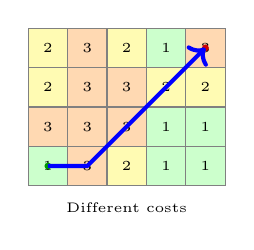
\begin{tikzpicture}[scale=0.5]
% Cost map grid
\foreach \x in {0,1,2,3,4} {
    \foreach \y in {0,1,2,3} {
        \pgfmathsetmacro{\cost}{int(1+random(0,2))}
        \ifnum\cost=1
            \fill[green!20] (\x,\y) rectangle ++(1,1);
        \fi
        \ifnum\cost=2
            \fill[yellow!30] (\x,\y) rectangle ++(1,1);
        \fi
        \ifnum\cost=3
            \fill[orange!30] (\x,\y) rectangle ++(1,1);
        \fi
        \node[font=\tiny] at (\x+0.5,\y+0.5) {\cost};
    }
}
\draw[step=1,gray] (0,0) grid (5,4);

\fill[green!60!black] (0.5,0.5) circle (2.5pt);
\fill[red!80!black] (4.5,3.5) circle (2.5pt);

\draw[blue, line width=1.5pt, ->] (0.5,0.5) -- (1.5,0.5) -- (2.5,1.5) -- (3.5,2.5) -- (4.5,3.5);

\node[below, font=\tiny] at (2.5,-0.2) {Different costs};
\end{tikzpicture}
\end{center}
\end{columns}

\vspace{0.2cm}

\begin{alertblock}{Data Structure}
Heap - \textit{"Sorting your Neighbor"}
\end{alertblock}
\end{frame}

\begin{frame}{A* Search: Directed Optimality}
\begin{block}{Heuristic-Guided Search}
$f(n) = g(n) + h(n)$ where $h(n)$ = estimated cost to goal

\vspace{0.2cm}

Heuristics: Euclidean or Manhattan distance
\end{block}

\vspace{0.2cm}

\begin{center}
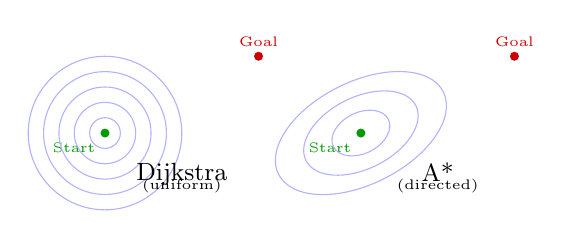
\begin{tikzpicture}[scale=0.65]
% Dijkstra (uniform)
\begin{scope}
\fill[green!60!black] (0,0) circle (2.5pt) node[below left, font=\tiny] {Start};
\fill[red!80!black] (3,1.5) circle (2.5pt) node[above, font=\tiny] {Goal};
\foreach \r in {0.3,0.6,0.9,1.2,1.5} {
    \draw[blue!30] (0,0) circle (\r);
}
\node[below, font=\small] at (1.5,-0.4) {Dijkstra};
\node[below, font=\tiny] at (1.5,-0.7) {(uniform)};
\end{scope}

% A* (directed)
\begin{scope}[xshift=5cm]
\fill[green!60!black] (0,0) circle (2.5pt) node[below left, font=\tiny] {Start};
\fill[red!80!black] (3,1.5) circle (2.5pt) node[above, font=\tiny] {Goal};
\draw[blue!30, rotate around={26.5:(0,0)}] (0,0) ellipse (1.8 and 1);
\draw[blue!30, rotate around={26.5:(0,0)}] (0,0) ellipse (1.2 and 0.7);
\draw[blue!30, rotate around={26.5:(0,0)}] (0,0) ellipse (0.6 and 0.4);
\node[below, font=\small] at (1.5,-0.4) {A*};
\node[below, font=\tiny] at (1.5,-0.7) {(directed)};
\end{scope}
\end{tikzpicture}
\end{center}

\vspace{0.2cm}

\begin{alertblock}{Advantage}
Fewer nodes expanded than Dijkstra
\end{alertblock}
\end{frame}

\begin{frame}{Weighted A*: Speed vs Optimality}
\begin{block}{The Epsilon Factor}
\textbf{Weighted A*:} $f(n) = g(n) + \epsilon \cdot h(n)$

where $\epsilon$ (epsilon) controls the greediness
\end{block}

\vspace{0.3cm}

\begin{columns}[T]
\column{0.45\textwidth}
\begin{exampleblock}{Epsilon Behavior}
\begin{itemize}
\item $\epsilon = 1$: Standard A* $\to$ Optimal
\item $\epsilon > 1$: Weighted A* $\to$ ``Greedy'' search $\to$ Faster but suboptimal
\item $\epsilon = 0$: Reduces to Dijkstra
\end{itemize}
\end{exampleblock}

\column{0.5\textwidth}
\begin{alertblock}{Real-Time Trade-off}
\textit{"Key technique for real-time planning"}

\vspace{0.2cm}

Fast ``good enough'' path in 10ms

vs

Perfect path in 1 second

\vspace{0.2cm}

For mobile robots, speed often matters more than perfection
\end{alertblock}
\end{columns}
\end{frame}

% ============================================================================
% ARTIFICIAL POTENTIAL FIELDS
% ============================================================================

\begin{frame}{Artificial Potential Fields: Continuous Planning}
\begin{block}{Physics Analogy}
\textbf{Concept:} Treat robot as a particle moving in an energy field

\vspace{0.2cm}

\textbf{Total Potential:}
\[U(q) = U_{att}(q) + U_{rep}(q)\]

\textbf{Control Force (gradient descent):}
\[F(q) = -\nabla U(q) = -\begin{bmatrix} \frac{\partial U}{\partial x} \\ \frac{\partial U}{\partial y} \end{bmatrix}\]
\end{block}

\vspace{0.3cm}

\begin{alertblock}{Operating Principle}
Robot ``rolls downhill'' toward goal while avoiding obstacles
\end{alertblock}
\end{frame}

\begin{frame}{Potential Field Components}
\begin{columns}[T]
\column{0.48\textwidth}
\begin{block}{Attractive Potential}
$U_{att}(q)$

\textbf{Purpose:}
\begin{itemize}
\item Pulls robot toward goal
\item Like spring/magnet
\item Increases with distance
\end{itemize}

$F_{att} = -\nabla U_{att}$

Points toward goal
\end{block}

\column{0.48\textwidth}
\begin{block}{Repulsive Potential}
$U_{rep}(q)$

\textbf{Purpose:}
\begin{itemize}
\item Pushes away from obstacles
\item Creates safety buffer
\item Limited range
\end{itemize}

$F_{rep} = -\nabla U_{rep}$

Points away from obstacles
\end{block}
\end{columns}

\vspace{0.3cm}

\begin{center}
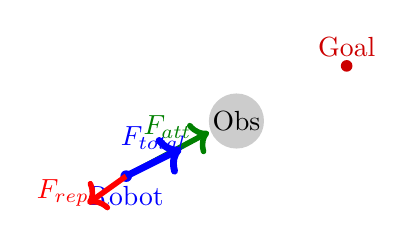
\begin{tikzpicture}[scale=0.7]
% Obstacle
\fill[gray!40] (3,2) circle (0.5);
\node at (3,2) {Obs};

% Robot
\fill[blue] (1,1) circle (3pt) node[below] {Robot};

% Goal
\fill[red!80!black] (5,3) circle (3pt) node[above] {Goal};

% Attractive force
\draw[->, green!50!black, line width=2pt] (1,1) -- (2.5,1.8);
\node[green!50!black, above] at (1.75,1.5) {$F_{att}$};

% Repulsive force
\draw[->, red, line width=2pt] (1,1) -- (0.3,0.5);
\node[red, left] at (0.5,0.7) {$F_{rep}$};

% Total force
\draw[->, blue, line width=2.5pt] (1,1) -- (2,1.5);
\node[blue, above] at (1.5,1.3) {$F_{total}$};
\end{tikzpicture}
\end{center}
\end{frame}

\begin{frame}{The Local Minima Problem}
\begin{alertblock}{The Trap}
$F_{total} = 0$ before goal - forces balance but robot stuck!
\end{alertblock}

\vspace{0.2cm}

\begin{center}
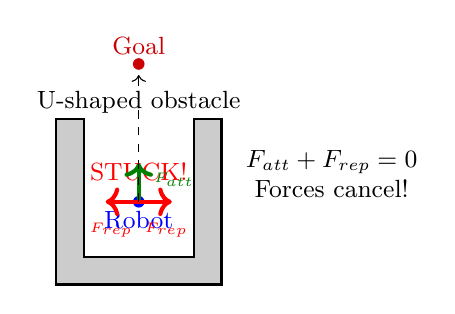
\begin{tikzpicture}[scale=0.7]
% U-shaped obstacle
\draw[fill=gray!40, thick] (1,0) -- (1,3) -- (1.5,3) -- (1.5,0.5) -- (3.5,0.5) -- (3.5,3) -- (4,3) -- (4,0) -- cycle;
\node[font=\small] at (2.5,3.3) {U-shaped obstacle};

% Robot stuck
\fill[blue] (2.5,1.5) circle (3pt) node[below, font=\small] {Robot};
\node[red, above, font=\small] at (2.5,1.7) {STUCK!};

% Forces
\draw[->, green!50!black, line width=1.5pt] (2.5,1.5) -- (2.5,2.2);
\node[green!50!black, right, font=\tiny] at (2.6,1.9) {$F_{att}$};

\draw[->, red, line width=1.5pt] (2.5,1.5) -- (1.9,1.5);
\draw[->, red, line width=1.5pt] (2.5,1.5) -- (3.1,1.5);
\node[red, below, font=\tiny] at (2,1.3) {$F_{rep}$};
\node[red, below, font=\tiny] at (3,1.3) {$F_{rep}$};

% Goal
\fill[red!80!black] (2.5,4) circle (3pt) node[above, font=\small] {Goal};
\draw[->, dashed] (2.5,1.5) -- (2.5,3.8);

% Balance
\node[align=center, font=\small] at (6,2) {$F_{att} + F_{rep} = 0$\\Forces cancel!};
\end{tikzpicture}
\end{center}

\vspace{0.2cm}

\begin{exampleblock}{Solutions}
\textit{"Random Walks"} - noise to escape; Multiple attempts
\end{exampleblock}
\end{frame}

\begin{frame}{Advanced Solution: Stein Variational Gradient Descent}
\begin{block}{Modern Approach}
\textbf{Stein Variational Gradient Descent (SVGD)}

Brief mention in lecture:
\begin{itemize}
\item Uses ``particle repulsion'' mechanism
\item Maintains multiple trajectory candidates
\item Prevents ``mode collapse''
\item Finds diverse paths simultaneously
\end{itemize}
\end{block}

\vspace{0.3cm}

\begin{alertblock}{Concept}
Instead of one path that gets stuck in local minimum, maintain multiple particles that repel each other - ensuring exploration of different solution modes
\end{alertblock}

\vspace{0.3cm}

\begin{exampleblock}{Application}
Mentioned as topic for advanced study / final projects
\end{exampleblock}
\end{frame}

% ============================================================================
% SYSTEM ARCHITECTURE
% ============================================================================

\begin{frame}{From Planning to Control: The $X \to U$ Problem}
\begin{alertblock}{The Disconnect}
\textbf{Planners output:} Positions/configurations $(x, y, \theta)$ - State $X$

\textbf{Robots need:} Control inputs $(v, \omega)$ or torques $\tau$ - Control $U$
\end{alertblock}

\vspace{0.3cm}

\begin{block}{Why The Gap Exists}
\begin{itemize}
\item \textbf{Non-holonomic constraints:} Differential-drive robot can't move sideways
\item \textbf{Dynamics:} Mass, inertia, friction ($F = ma$)
\item \textbf{Actuator limits:} Maximum speed, acceleration bounds
\item \textbf{Real-time requirements:} Must react to dynamic obstacles
\end{itemize}
\end{block}

\vspace{0.3cm}

\begin{exampleblock}{Solution}
Hierarchical architecture bridging geometric planning and physical control
\end{exampleblock}
\end{frame}

\begin{frame}{Hierarchical Planning Architecture}
\begin{center}
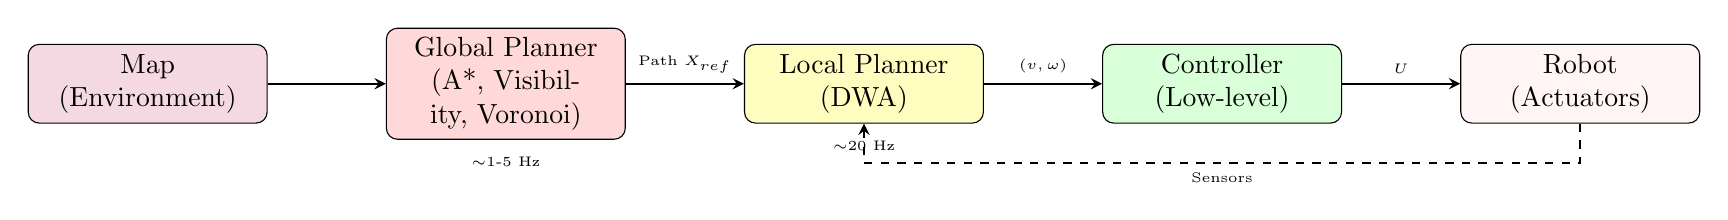
\begin{tikzpicture}[
    node distance=1.5cm,
    block/.style={rectangle, draw, fill=blue!20, text width=2.8cm, text centered, rounded corners, minimum height=1cm},
    arrow/.style={->, >=stealth, thick}
]
\node[block, fill=purple!15] (map) {Map\\(Environment)};
\node[block, fill=red!15, right=of map] (global) {Global Planner\\(A*, Visibility, Voronoi)};
\node[block, fill=yellow!25, right=of global] (local) {Local Planner\\(DWA)};
\node[block, fill=green!15, right=of local] (controller) {Controller\\(Low-level)};
\node[block, fill=pink!15, right=of controller] (robot) {Robot\\(Actuators)};

\draw[arrow] (map) -- (global);
\draw[arrow] (global) -- node[above, font=\tiny] {Path $X_{ref}$} (local);
\draw[arrow] (local) -- node[above, font=\tiny] {$(v, \omega)$} (controller);
\draw[arrow] (controller) -- node[above, font=\tiny] {$U$} (robot);
\draw[arrow, dashed] (robot.south) -- ++(0,-0.5) -| node[near start, below, font=\tiny] {Sensors} (local.south);

\node[below=0.1cm of global, font=\tiny] {$\sim$1-5 Hz};
\node[below=0.1cm of local, font=\tiny] {$\sim$20 Hz};
\end{tikzpicture}
\end{center}

\vspace{0.3cm}

\begin{columns}[T]
\column{0.33\textwidth}
\begin{block}{Global Planner}
\begin{itemize}\small
\item Low frequency
\item Solves the ``maze''
\item Strategic path
\item Ignores dynamics
\end{itemize}
\end{block}

\column{0.33\textwidth}
\begin{block}{Local Planner}
\begin{itemize}\small
\item High frequency
\item Dynamic obstacles
\item Feasible velocities
\item Example: DWA
\end{itemize}
\end{block}

\column{0.33\textwidth}
\begin{block}{Controller}
\begin{itemize}\small
\item Highest frequency
\item Motor commands
\item Physical execution
\item Handles dynamics
\end{itemize}
\end{block}
\end{columns}
\end{frame}

\begin{frame}{Dynamic Window Approach (DWA)}
\begin{block}{Local Planning in Velocity Space}
\textit{"Image Action" architecture mentioned in notes}

\textbf{Core Concept:} Search in velocity space $(v, \omega)$ instead of position space

\textbf{Dynamic Window:} Reachable velocities given acceleration limits
\begin{itemize}
\item $V \in [V_t - a_{max} \cdot dt, V_t + a_{max} \cdot dt]$
\item $\Omega \in [\omega_t - \alpha_{max} \cdot dt, \omega_t + \alpha_{max} \cdot dt]$
\end{itemize}
\end{block}

\vspace{0.3cm}

\begin{exampleblock}{Process}
\begin{enumerate}
\item Sample velocity pairs $(v_i, \omega_i)$ within dynamic window
\item Simulate forward trajectory for each pair
\item Evaluate cost: heading + clearance + velocity
\item Select optimal $(v^*, \omega^*)$
\item Execute for short time, then replan
\end{enumerate}
\end{exampleblock}
\end{frame}

% ============================================================================
% HISTORICAL CONTEXT
% ============================================================================

\begin{frame}{Historical Context: Industrial Origins}
\begin{block}{Where These Methods Come From}
\textit{"A lot of these deterministic methods come from robot manipulators and industry"}
\end{block}

\vspace{0.3cm}

\begin{columns}[T]
\column{0.48\textwidth}
\begin{exampleblock}{Industrial Robot Context}
\begin{itemize}
\item 4-6+ degrees of freedom arms
\item More complex than mobile robots
\item \textbf{BUT:} Static environments
\item Planning happens once
\item High efficiency crucial
\end{itemize}

\textit{"Highly efficient compared to probabilistic methods"}
\end{exampleblock}

\column{0.48\textwidth}
\begin{alertblock}{Mobile Robot Challenge}
\textit{"These methods cannot be used for dynamic environment"}

\begin{itemize}
\item Dynamic obstacles
\item Unknown environments
\item Need reactive planning
\item Real-time constraints
\end{itemize}

\textit{"A lot of modifications happen to apply them for mobile robot use cases"}
\end{alertblock}
\end{columns}
\end{frame}

% ============================================================================
% SUMMARY
% ============================================================================

\begin{frame}{Method Selection Guide}
\begin{center}
\begin{tabular}{lccc}
\toprule
\textbf{Method} & \textbf{Optimality} & \textbf{Safety} & \textbf{Best For} \\
\midrule
Visibility Graph & $\checkmark\checkmark$ & $\times$ & Static, optimal paths needed \\
Voronoi Diagram & $\times$ & $\checkmark\checkmark$ & Uncertainty, safety critical \\
Grid/Cell Decomp & $\sim$ & $\sim$ & Simple environments, known maps \\
RRT (Probabilistic) & $\times$ & $\sim$ & High DOF, complex spaces \\
\bottomrule
\end{tabular}
\end{center}

\vspace{0.3cm}

\begin{block}{Search Algorithm Trade-offs}
\begin{itemize}
\item \textbf{BFS/DFS:} Simple but inefficient for large spaces
\item \textbf{Dijkstra:} Optimal but slow (searches all directions)
\item \textbf{A*:} Optimal and efficient with good heuristic
\item \textbf{Weighted A*} ($\epsilon > 1$): Fast but suboptimal - real-time preference
\end{itemize}
\end{block}
\end{frame}

\begin{frame}{Key Takeaways}
\begin{enumerate}
\item \textbf{Probabilistic vs Deterministic}
\begin{itemize}
\item Time guarantees vs dimensional complexity
\item RRT for high-DOF, deterministic for mobile robots
\end{itemize}

\item \textbf{Graph Construction Determines Path Quality}
\begin{itemize}
\item Visibility: Optimal but risky
\item Voronoi: Safe but longer
\item Design choice based on requirements
\end{itemize}

\item \textbf{Search Algorithms: Speed vs Optimality}
\begin{itemize}
\item Weighted A* gives control over trade-off
\item Real-time often prefers ``good enough'' quickly
\end{itemize}

\item \textbf{Planning $\neq$ Control}
\begin{itemize}
\item Hierarchical architecture bridges the gap
\item Global strategy + local reactivity + physical execution
\end{itemize}
\end{enumerate}
\end{frame}

\begin{frame}{Industry Challenges Ahead}
\begin{alertblock}{Current Bottlenecks}
\begin{itemize}
\item \textbf{Map dependency:} High-definition maps expensive to create/maintain
\item \textbf{Computational load:} Real-time planning still computationally heavy
\item \textbf{Operational cost:} \textit{"Operation of autonomous cars still very challenging"}
\end{itemize}
\end{alertblock}

\vspace{0.3cm}

\begin{exampleblock}{Future Directions}
\begin{itemize}
\item Truly mapless navigation
\item Lighter computational requirements
\item Better integration of planning and control
\item \textit{"Tons of optimization space in that ecosystem"}
\end{itemize}
\end{exampleblock}
\end{frame}

\begin{frame}{Final Perspective}
\begin{block}{No Single ``Best'' Method}
\textit{"Based on the situation and the problem you are solving..."}

\vspace{0.2cm}

The right planner depends on:
\begin{itemize}
\item Dimensionality of configuration space
\item Static vs dynamic environment
\item Optimality requirements
\item Computational resources
\item Safety criticality
\item Real-time constraints
\end{itemize}
\end{block}

\vspace{0.3cm}

\begin{center}
\Large
\textbf{Understanding the trade-offs enables intelligent method selection}
\end{center}
\end{frame}

\begin{frame}{Homework}
\begin{block}{Plotting Potential Fields}
Implement potential fields showing two scenarios:
\begin{itemize}
\item One where the robot successfully navigates from A to B,
\item One where it fails
\end{itemize}
\end{block}
\end{frame}

\begin{frame}{Questions?}
\begin{center}
\vspace{1cm}
\Large
\textbf{Next Lecture: Advanced Planning Topics}
\end{center}
\end{frame}

\end{document}
